%% Journal of Systems and Software regular research article

\documentclass[a4paper,fleqn]{cas-dc}

\usepackage[authoryear,longnamesfirst]{natbib}

% British English is required throughout this manuscript.
% No ORCID identifiers were supplied in the authoritative previous manuscript.
\let\printorcid\relax

\begin{document}

\shorttitle{Contextual Input and Shared Representation}
\shortauthors{A. Kadouma et al.}

\title[mode=title]{Evaluating Contextual Input and Shared Representation in Multi-Metric Runtime Forecasting for Cloud Software Systems}

\author[1]{Abdelhak Kadouma}
\cormark[1]
\ead{abdelhak.kadouma@uwasa.fi}
\credit{Conceptualization, Methodology, Software, Data curation, Formal analysis, Validation, Visualization, Writing -- original draft}

\author[1]{Amit Shukla}
\ead{amit.shukla@uwasa.fi}
\credit{Supervision, Conceptualization, Methodology, Writing -- review \& editing}

\author[1]{Mohammed Elmusrati}
\ead{moel@uwasa.fi}
\credit{Supervision, Project administration, Writing -- review \& editing}

\affiliation[1]{
  organization={University of Vaasa},
  city={Vaasa},
  country={Finland}
}

\cortext[1]{Corresponding author}

\begin{abstract}
Multi-metric runtime forecasting requires decisions about other-resource
telemetry and cross-target representation sharing, with consequences for
accuracy and per-entity model consolidation. Our frozen experiment compares
conventional long short-term memory (LSTM) formulations: S1 uses own-resource
input and independent target models; S2 uses all-resource input and
independent target models; M1 uses all-resource input and a shared
multi-resource model. We evaluate central processing unit (CPU) utilisation,
throughput, memory and disk-write activity across TimeTrack development data,
Bitbrains fastStorage and Rnd external environments, and Materna T1--T3
dependent temporal blocks. Separate post-hoc controls constrain S2 to
M1-selected contexts and increase M1's hidden size from H64 to H129 to
approximately match S2's aggregate parameter count. A matched-context
comparison of Ridge autoregression (AR) and autoregression with cross-resource
inputs (ARX) examines contextual value beyond LSTMs. Contextual value is
selective and model- and environment-dependent; memory benefits recur but
are not universal. Adverse M1:S2 throughput, memory and disk-write point
estimates persist across all six blocks under both controls, without
identifying sharing alone as the cause. Yet M1 matched-cell median MAE ratios
are close to one in many comparisons, and some larger MacroMAE penalties are
tail-concentrated. Per-entity consolidation therefore presents a
target-specific accuracy--consolidation trade-off. Ridge indicates
model-family dependence. Effects can change sign across the recorded seeds,
and sign stability need not imply magnitude stability. Relative gains do not
ensure superiority to persistence. Contextual input and representation
sharing require separate, resource-specific evaluation.
\end{abstract}

\begin{keywords}
runtime forecasting \sep
cloud telemetry \sep
multi-metric forecasting \sep
multi-task learning \sep
contextual input \sep
shared representations
\end{keywords}

\maketitle

\section{Introduction}
\label{sec:introduction}

Cloud telemetry forecasting can inform adaptation and resource management
\citep{Taherizadeh2018Monitoring,Bauer2020SelfAware}.
Engineers must decide whether a target's forecaster should include other
resources' telemetry and whether several targets should share a predictive
representation. These choices change input information and model organisation,
respectively. Consolidation reduces the models to manage but need not improve
every resource's forecast. We evaluate accuracy and model consolidation,
not downstream control effectiveness.

Established runtime-series benchmarking spans
classical statistical, neural and zero-shot foundation models
\citep{DiMenna2026RuntimeForecasting}. Cloud studies include multivariate
resource inputs, recurrent architectures, joint multi-output prediction and
hybrid models evaluated across multiple provider environments
\citep{Ullah2023CloudBiLSTM,Tripathi2025MMRP}. Global forecasting also learns
parameters across collections of series \citep{Salinas2020DeepAR}.
These precedents motivate empirical design choices for particular resource
targets, not a new forecasting architecture.

\emph{Contextual input} supplies other resources' histories to a target model
without requiring shared parameters. \emph{Representation sharing} learns
several targets jointly. Multi-task learning
offers inductive transfer through related tasks \citep{Caruana1997Multitask},
but task combinations and sharing arrangements require evaluation
\citep{Standley2020TaskGrouping,Fifty2021TaskGroupings,Nochumsohn2025MTLinear}.
Independent all-input target models provide an intermediate comparison
between own-resource and shared forecasting. MMRP already compares
univariate/multivariate single-target CPU and memory forecasting
\citep{Tripathi2025MMRP}; our bounded contribution is the within-study
comparison including this intermediate organisation and joint resource
forecasting (Section~\ref{sec:rw-gap}).

We evaluate conventional LSTM formulations with independent target models
using own-resource histories (S1) or all-resource histories (S2), and a shared
representation with resource-specific heads using all-resource histories
(M1). S2 versus S1 evaluates contextual information, M1 versus S2 the
implemented shared-LSTM transition, and M1 versus S1 the complete joint
system. The evaluated resources are CPU utilisation, throughput, memory usage
and disk-write activity. TimeTrack supplies development evidence, Bitbrains
fastStorage and Rnd provide external environments, and Materna T1--T3 provide
dependent temporal replication. The comparisons retain source-specific
eligible populations and evaluation protocols.
Sections~\ref{sec:framework} and~\ref{sec:methodology} define the original
formulations and evaluation.

The four questions in Section~\ref{sec:research-questions} address contextual
input (RQ1), the operational shared-LSTM contrast (RQ2), the complete joint
system (RQ3), and heterogeneity and accuracy--efficiency trade-offs (RQ4).

Post-hoc sensitivity controls impose M1-selected contexts on S2, increase M1
from H64 to H129 to approximately match S2's aggregate capacity, and compare
Ridge autoregression (AR) with cross-resource autoregression (ARX) at matched
contexts. Section~\ref{sec:posthoc-controls} details their separate selection
procedures and limits; they qualify, rather than replace, the frozen results.

Contextual value is selective: memory shows recurring benefits, but directions
depend on model family and environment. M1:S2 throughput, memory and disk-write
point estimates remain adverse in all six blocks under both separate LSTM
controls, without identifying sharing alone as the cause. Matched-cell median
M1/S2 MAE ratios are close to one in many comparisons, whereas some much larger
MacroMAE penalties are tail-concentrated (Section~\ref{sec:results-rq2}).
Per-entity consolidation can therefore offer a target-specific trade-off,
subject to assessment of adverse tails. Original external
H64 M1 uses approximately $74.5\%$ fewer parameters and $75\%$ fewer models per
target set. Seed sensitivity and poor persistence skill in some settings bound
this accuracy--consolidation trade-off, which establishes no production savings
(Section~\ref{sec:cross-dataset-synthesis}). We make four contributions:

\begin{enumerate}
  \item We evaluate S1/S2/M1 operational contrasts that distinguish
    contextual-input value from the accuracy consequences of the implemented
    shared-LSTM design and its model consolidation.
  \item We characterise resource-, environment- and model-dependent contextual
    value using the original LSTM comparison and a post-hoc matched-context
    Ridge AR/ARX comparison across all six evidence blocks.
  \item We test the robustness of the shared-LSTM contrast with separate
    common-context and H129 approximate aggregate-capacity controls,
    distinguishing persistent adverse point estimates from causal claims
    about representation sharing alone.
  \item We relate forecasting accuracy to model-management choices while
    bounding conclusions by matched-cell behaviour, existing-seed sensitivity,
    persistence skill and the eligible populations studied.
\end{enumerate}

\section{Related Work}
\label{sec:related-work}

\subsection{Runtime and Cloud-Resource Forecasting}
\label{sec:rw-runtime}

Runtime telemetry supports configuration and resource-management decisions in
cloud and self-adaptive software systems
\citep{Taherizadeh2018Monitoring,Bauer2020SelfAware}. Prediction-based
provisioning and service-quality forecasting already connect forecast accuracy
with software design
\citep{Calheiros2015ARIMA,Syu2017DynamicQoS}. Forecast quality nevertheless
differs from controller effectiveness: policies, actuation delays and
uncertainty also affect operational outcomes \citep{Qu2018Autoscaling}.
Here the engineering question concerns input selection and model management,
not a measured autoscaling or service-level benefit.

The relevant literature spans different prediction organisations.
\citet{DiMenna2026RuntimeForecasting} compare model families on application
runtime metrics, fitting conventional models independently per series and
applying foundation models zero-shot to individual histories. In contrast,
\citet{Ullah2023CloudBiLSTM} use ten-channel histories and joint ten-channel
forecasts with a common BiLSTM representation on fastStorage and Rnd.
Multivariate covariates, hybrid resource predictors, joint outputs and
multi-provider evaluation are established capabilities
\citep{Tran2018MultivariateFuzzy,Xu2022esDNN,Tripathi2025MMRP,
Rossi2025CloudUncertainty,Zhang2025SWTCLSTM}, alongside online resource and
microservice-indicator forecasting \citep{Gao2026OMCR,Gao2026MaMiClif}.
These precedents motivate comparing design choices, not claiming a new
forecasting architecture.

TimeTrack provides OAI CI/CD telemetry with reported resource correlations
\citep{Meliani2025TimeTrack}. These motivate contextual inputs, but do not
establish predictive value conditional on the target's own history.
That value requires a forecasting comparison, not correlation alone.

\subsection{Information Scope and Sharing in Forecasting}
\label{sec:rw-information-sharing}

Input channels, output targets and parameter sharing are separate choices.
A model may use several resource histories for one target; a vector output
may represent several horizons of that same target rather than several
resources. Independent target models require separate fitted parameters,
not merely separate output values or separately processed channels.

MMRP directly compares univariate and multivariate single-target forecasts
\citep{Tripathi2025MMRP}. Its CPU and memory results are reported separately;
the exact all-channel assignment and independent-fit inventory are not fully
specified. It is a substantive S1--S2-related precedent, not a reported joint
resource-sharing arm. Likewise, esDNN uses resource covariates for CPU
prediction \citep{Xu2022esDNN}. Neither multichannel input nor multi-head
attention by itself establishes cross-target parameter sharing. Ullah's joint
BiLSTM does share a representation, but its reported architecture comparisons
do not include an independent all-input target-model bridge.

The distinction also matters outside cloud telemetry. PatchTST processes
channels independently while reusing embedding and Transformer weights across
them \citep{Nie2023PatchTST}. Channel independence therefore does not mean
independently fitted models. In contrast, iTransformer represents individual
variates as tokens and models relationships between them through attention
\citep{Liu2024iTransformer}.
DeepAR and local/global forecasting share functions across series rather than
necessarily presenting all series as simultaneous covariates
\citep{Salinas2020DeepAR,MonteroManso2021GlobalForecasting}.
These distinctions matter when deciding whether telemetry should be added to
a predictor or target models should be consolidated.

\subsection{Multi-Task Learning, Task Relatedness, and Adverse Transfer}
\label{sec:rw-multitask}

Shared learning can provide an inductive bias \citep{Caruana1997Multitask},
but its value depends on tasks, data and sharing structure
\citep{Yu2025MultitaskFundamentals}. Task grouping explicitly examines which
tasks should learn together under accuracy and computational constraints
\citep{Standley2020TaskGrouping,Fifty2021TaskGroupings}.
Multi-objective and gradient-modification methods address conflicting updates
\citep{Sener2018MultiObjective,Yu2020GradientSurgery}. These are established
responses to adverse transfer, not evidence of a measured mechanism in our
resource forecasters.

\citet{Nikentari2022NARMAXLSTM} provide a forecasting precedent:
NARMAX-LSTM combines lagged station inputs, shared LSTM layers and
station-specific outputs, compares single-task baselines and discusses
negative transfer. Its network-reduction argument is qualitative,
and an independent all-input target-model bridge is not established.
MTLinear assigns temporal weights to variate groups, analyses gradient
conflicts and balance, and evaluates grouping, parameter size and computation
\citep{Nochumsohn2025MTLinear}. Applying common temporal weights to each
variate's own history differs from mixing contextual channels. Its grouping
endpoints inform independent-versus-shared learning without reproducing our
all-input S2--M1 contrast.

Cloud multi-task forecasting also predates this study:
\citet{Bi2019CloudMultitask} combine workload decomposition with stochastic
configuration networks and report training-speed comparisons. The inspected
evidence does not establish equivalence to resource-target sharing or an
all-input independent baseline. Efficiency evidence must therefore be
distinguished from a measured target-model consolidation trade-off.
MMRP's inference-throughput measurements and Di Menna's model-size and
adaptation-cost discussion likewise provide efficiency-related evidence,
without the same target-consolidation analysis.
Table~\ref{tab:related-work-comparison} distinguishes these forms.
Negative transfer and forecasting efficiency are not novel topics introduced here.

\subsection{Evaluation Gap and Study Scope}
\label{sec:rw-gap}

The contribution concerns the within-study comparison, not an architecture
or literature-wide priority claim. The inspected studies establish contextual
single-target forecasting, shared forecasting, adverse-transfer analysis and
efficiency evaluation in different designs. Table~\ref{tab:related-work-comparison}
records their overlap and evidence limits rather than certifying an absence
across the literature.

% Cell-level provenance is retained in review_revision/stage19e_evidence.
\begin{table*}[t]
  \caption{Closest inspected designs: contextual inputs, target sharing and
  model-management evidence. Codes describe reported designs under the
  definitions below, not architectural equivalence or a priority ranking.}
  \label{tab:related-work-comparison}
  \centering
  \small
  \setlength{\tabcolsep}{3pt}
  \begin{tabular}{@{}
    >{\raggedright\arraybackslash}p{0.180\textwidth}
    >{\raggedright\arraybackslash}p{0.200\textwidth}
    *{2}{>{\raggedright\arraybackslash}p{0.105\textwidth}}
    *{2}{>{\raggedright\arraybackslash}p{0.100\textwidth}}
    >{\raggedright\arraybackslash}p{0.130\textwidth}@{}}
    \toprule
    Study & Contextual input / target organisation
      & Independent all-input targets & Shared cross-target parameters
      & Single-task vs shared comparison & Adverse-transfer analysis
      & Efficiency / consolidation evidence \\
    \midrule
    \citet{Ullah2023CloudBiLSTM}
      & YES; ten-channel histories to joint ten-channel forecasts.
      & NO & YES; common BiLSTM & NO & NO
      & PARTIAL; qualitative training discussion \\
    \addlinespace
    \citet{DiMenna2026RuntimeForecasting}
      & NO; individual metric histories to same-metric horizons.
      & NO & NO; pretrained reuse is a different axis & NO & NO
      & PARTIAL; sizes and cost discussion \\
    \addlinespace
    \citet{Tripathi2025MMRP} (MMRP)
      & YES; own/multichannel histories to one target.
      & PARTIAL; exact channel/fit inventory unspecified
      & NO & NO & NO
      & PARTIAL; inference throughput \\
    \addlinespace
    \citet{Nikentari2022NARMAXLSTM} (NARMAX-LSTM)
      & YES; lagged station inputs to station targets.
      & Not established & YES; shared LSTM layers
      & YES; single-task baselines & YES; task-wise discussion
      & PARTIAL; network-reduction argument \\
    \addlinespace
    \citet{Nochumsohn2025MTLinear} (MTLinear)
      & NO channel mixing in the linear predictor; own histories, grouped targets.
      & NO & YES; weights within groups
      & PARTIAL; grouping endpoints & YES; gradient analysis
      & YES; parameter/grouping and compute analysis \\
    \addlinespace
    \citet{Bi2019CloudMultitask}
      & Not established for cross-resource inputs; decomposed workload.
      & Not established & Not established for resource targets
      & Not established & Not established
      & PARTIAL; training-speed comparison \\
    \addlinespace
    This study
      & YES; S1 own history; S2/M1 all histories; independent/joint resource targets.
      & YES; S2 & YES; M1 encoder & YES; S2--M1
      & YES; operational accuracy contrast
      & YES; model and parameter counts; worker fit-hours \\
    \bottomrule
  \end{tabular}

  \vspace{2pt}
  \parbox{\textwidth}{\footnotesize
    Contextual input means other variables enter a target's predictor, not
    merely that a dataset is multivariate. Independent all-input targets means
    separately fitted target models with the selected multichannel inputs.
    Sharing concerns learning across target series, not horizons alone or
    pretrained reuse. YES: explicit evidence; NO: excluded by the inspected
    reported design; PARTIAL: related, limited or incompletely matched evidence.
    Not established: available evidence does not settle the cell.
    Single-task/shared comparisons need not hold inputs or architecture fixed;
    adverse-transfer analysis coded YES means explicit empirical analysis of
    adverse-transfer outcomes, not causal identification of the mechanism.
    Efficiency PARTIAL covers timing, qualitative cost or network-reduction
    evidence without the quantified parameter/grouping or consolidation analysis
    coded YES. No code rules out unpublished implementations.}
\end{table*}


S2 is the intermediate operational control: each target model receives all
resource histories but retains separate fitted parameters. S1--S2 examines
additional contextual input; S2--M1 examines the implemented move to a shared
resource predictor. Capacity, optimisation and selected settings also differ,
so these are not pure causal interventions or a complete $2\times2$ design.
Separate post-hoc common-context and H129 capacity controls qualify that
contrast, while matched-context Ridge AR/ARX checks contextual directions in
another model family (Section~\ref{sec:posthoc-controls}).

The same operational contrasts are retained through TimeTrack development,
the separate fastStorage and Rnd external environments, and dependent Materna
T1--T3 temporal blocks. Resource-wise accuracy, local model consolidation and
eligible-population limits define the evidence contribution. This supports
runtime forecasting and model-management choices without claiming independent
Materna datasets, a universal transfer mechanism or superiority to untested
architectures. Section~\ref{sec:framework} defines the formulations.

\section{Multi-Metric Runtime Forecasting Framework}
\label{sec:framework}

The framework distinguishes access to resource histories from sharing a
learned predictive representation across resource targets.
Figure~\ref{fig:sharing-framework} summarises S1, S2 and M1 and their matched
operational contrasts.

\begin{figure*}[t]
  \centering
  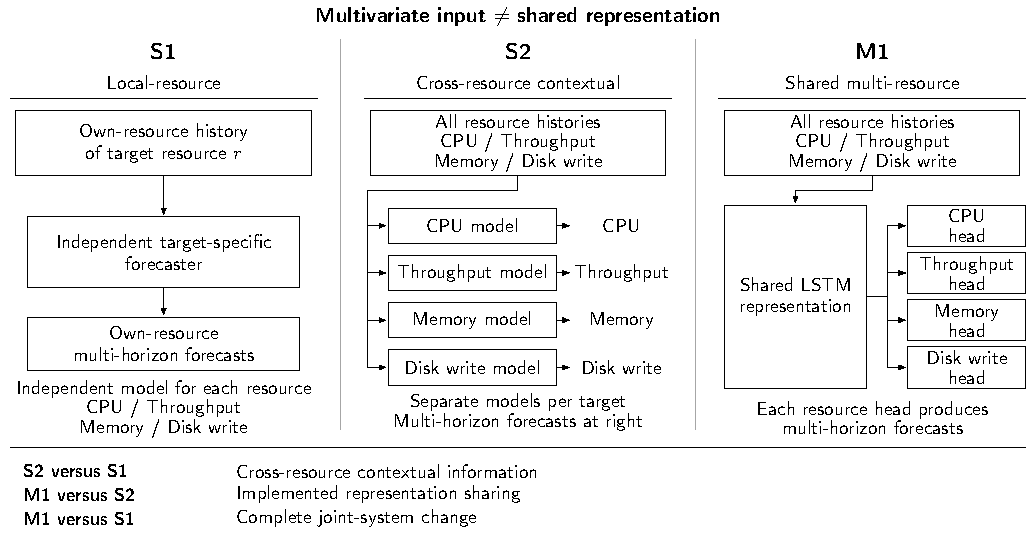
\includegraphics[width=\textwidth]{figures/framework_s1_s2_m1.pdf}
  \caption{S1 fits independent target models from own-resource histories;
  S2 supplies all histories to each independently trained target model.
  M1 uses all histories with a shared LSTM representation and resource-specific
  heads. S2 versus S1 assesses contextual input; M1 versus S2 the implemented
  move to representation sharing; M1 versus S1 the complete joint-system
  change. Models are fitted separately for each entity, outer fold and seed;
  S1/S2 use four networks per target set and M1 uses one joint network.
  These are matched operational comparisons, not a complete
  $2\times2$ design, parameter-matched interventions or pure causal
  isolation of either design choice.}
  \label{fig:sharing-framework}
\end{figure*}

\subsection{Problem Formulation}
\label{sec:problem}

Let $\mathcal{R}=\{\mathrm{cpu},\mathrm{thr},\mathrm{mem},\mathrm{disk}\}$
denote the resource set and let $R=|\mathcal{R}|=4$. At discrete time $t$,
the multivariate telemetry observation is
$\mathbf{x}_t=(x_t^{(r)})_{r\in\mathcal{R}}\in\mathbb{R}^{R}$. For a context
length $L\in\mathbb{N}$, the complete history available at forecasting origin
$t$ is
\begin{equation}
  \mathbf{X}_{t,L}
  = [\mathbf{x}_{t-L+1},\ldots,\mathbf{x}_{t}]^{\mathsf T}
  \in \mathbb{R}^{L\times R}.
  \label{eq:multiresource-context}
\end{equation}
Let $\mathcal{H}\subset\mathbb{N}_{>0}$ be a finite set of forecast horizons.
For target resource $r$, $y_{t+h}^{(r)}$ is the future target at horizon
$h\in\mathcal{H}$ and
$\mathbf{y}_{t,\mathcal{H}}^{(r)}=(y_{t+h}^{(r)})_{h\in\mathcal{H}}$ is its
multi-horizon target vector. A forecaster produces
\begin{equation}
  \widehat{\mathbf{y}}_{t,\mathcal{H}}^{(r)}
  = F_r(\mathcal{I}_{t,L};\boldsymbol{\theta}),
  \label{eq:forecasting-task}
\end{equation}
where $\mathcal{I}_{t,L}$ denotes the formulation-dependent information set
and $\boldsymbol{\theta}$ denotes the relevant model parameters.

Models are entity-specific: for each TimeTrack machine or external VM,
outer fold and seed, S1/S2 fit four target-specific networks and M1 one joint
four-resource network. M1 shares across that entity's targets, never across
entities. These local model-complement counts exclude the separate
candidate-context inner fits and final refits; they do not describe a
globally deployed four-versus-one system.

Contexts contain aligned observations available at or before $t$; targets lie
strictly afterwards. Horizons use each dataset's time grid, preserving temporal
order without requiring a universal sampling interval. Eligible origins supply
every formulation's inputs and complete targets. Matched origins, targets,
horizons and partitions prevent sample differences from changing a contrast.

\subsection{Resource Metrics and Multi-Horizon Forecasting}
\label{sec:resource-horizons}

The resource vector comprises CPU utilisation, aggregate throughput, memory
usage, and disk-write activity. CPU utilisation represents processor demand;
throughput represents the aggregate rate of data transferred through the
runtime environment; memory usage represents occupied memory; and disk-write
activity represents write traffic to persistent storage. Dataset-specific
fields, units and sampling intervals are mapped in Section~\ref{sec:datasets}.

Each formulation jointly predicts its full horizon vector, so output
organisation is fixed rather than changed from single- to multi-horizon
training. Contexts $L$ and finite positive offsets $\mathcal{H}$ are fixed
before evaluation but may vary with source cadence without changing the
formulation definitions. Distinct resources may supply predictive context;
varying access to their histories tests this while keeping targets fixed.
Resource-specific training transforms and scaling accommodate different
distributions and optimisation scales; evaluation returns forecasts to native
units (Section~\ref{sec:preprocessing}).

\subsection{S1 Local-Resource Forecasting}
\label{sec:s1}

S1 is the local-information formulation. For target resource $r$, its input is
the single-channel sequence
\begin{equation}
  \mathbf{X}_{t,L}^{\mathrm{S1},r}
  = [x_{t-L+1}^{(r)},\ldots,x_t^{(r)}]^{\mathsf T}
  \in\mathbb{R}^{L\times 1},
  \label{eq:s1-input}
\end{equation}
and its output is
\begin{equation}
  \widehat{\mathbf{y}}_{t,\mathcal{H}}^{(r)}
  = f_r^{\mathrm{S1}}
    (\mathbf{X}_{t,L}^{\mathrm{S1},r};\boldsymbol{\theta}_r^{\mathrm{S1}})
  \in\mathbb{R}^{|\mathcal{H}|}.
  \label{eq:s1-forecast}
\end{equation}
A distinct parameter set $\boldsymbol{\theta}_r^{\mathrm{S1}}$ gives each
resource its own encoder, prediction mapping and objective. S1 is the
multi-horizon local-history baseline within the common model family;
withholding non-target channels does not assume resource independence.

\subsection{S2 Cross-Resource Contextual Forecasting}
\label{sec:s2}

S2 expands the information set while retaining target-specific modelling. For
every $r\in\mathcal{R}$, the input is the complete history
\begin{equation}
  \mathbf{X}_{t,L}^{\mathrm{S2},r}=\mathbf{X}_{t,L}
  \in\mathbb{R}^{L\times R},
  \qquad
  \widehat{\mathbf{y}}_{t,\mathcal{H}}^{(r)}
  = f_r^{\mathrm{S2}}
    (\mathbf{X}_{t,L};\boldsymbol{\theta}_r^{\mathrm{S2}}).
  \label{eq:s2-forecast}
\end{equation}
Each $\boldsymbol{\theta}_r^{\mathrm{S2}}$ is trained independently.
Non-target histories act as covariates, but the output and loss remain
specific to $r$: gradients from one target cannot update another model's
representation. Thus all-resource input does not establish shared learning
across targets.

Under matched support, S2 versus S1 evaluates contextual input while retaining
separate models, without presuming that extra channels are informative or
that their contribution has a particular sign.

\subsection{M1 Shared Multi-Resource Forecasting}
\label{sec:m1}

M1 combines all-resource input with a representation shared across target
tasks. A temporal encoder $E_{\boldsymbol{\theta}}$ maps the complete context
to a latent vector $\mathbf{z}_t$, and one resource-specific head
$g_{r,\boldsymbol{\phi}_r}$ maps that representation to the horizon vector for
resource $r$:
\begin{equation}
  \begin{aligned}
    \mathbf{z}_t
      &= E_{\boldsymbol{\theta}}(\mathbf{X}_{t,L}), \\
    \widehat{\mathbf{y}}_{t,\mathcal{H}}^{(r)}
      &= g_{r,\boldsymbol{\phi}_r}(\mathbf{z}_t),
      && r\in\mathcal{R}.
  \end{aligned}
  \label{eq:m1-forecast}
\end{equation}
The resulting output has resource-by-horizon structure
$\widehat{\mathbf{Y}}_{t}\in\mathbb{R}^{R\times|\mathcal{H}|}$.
The common encoder is updated by all resource losses; head gradients update
only the corresponding head, retaining resource-specific predictive mappings.
This single multi-output model introduces no attention, gating, task routing
or adaptive sharing.

Let $\mathcal{B}$ be a training mini-batch, and let
$\widetilde{y}_{i,h}^{(r)}$ and
$\widehat{\widetilde{y}}_{i,h}^{(r)}$ denote the scaled target and prediction
for sample $i$, resource $r$, and horizon $h$. M1 uses the equally weighted
scaled-space objective
\begin{equation}
  \mathcal{L}_{\mathrm{M1}}
  = \frac{1}{|\mathcal{B}|R|\mathcal{H}|}
    \sum_{i\in\mathcal{B}}
    \sum_{r\in\mathcal{R}}
    \sum_{h\in\mathcal{H}}
    \left(
      \widehat{\widetilde{y}}_{i,h}^{(r)}
      - \widetilde{y}_{i,h}^{(r)}
    \right)^2.
  \label{eq:m1-loss}
\end{equation}
This is the arithmetic mean of four transformed/robust-scaled resource MSEs,
with equally weighted horizons. S1/S2 use the corresponding single-resource
MSE. Equal coefficients do not imply equal realised losses or gradients:
residual distributions and derivatives differ. No task weights are learned
and no resource is conditionally suppressed. Scaling is training-only
(Section~\ref{sec:preprocessing}).

\subsection{Controlled Information-Sharing Decomposition}
\label{sec:decomposition}

The three matched operational formulations define three comparisons, each evaluated for the same
resource, horizon, and matched support. Let $Q(F)$ denote a lower-is-better
error functional for formulation $F$ under such a fixed evaluation unit. For
a baseline $A$ and candidate $B$, define the signed error reduction
\begin{equation}
  D_Q(A\rightarrow B)=Q(A)-Q(B),
  \label{eq:controlled-reduction}
\end{equation}
so that a positive value indicates lower error for $B$. Exact metric,
aggregation, and percentage-normalisation rules are specified in the
experimental methodology. The framework-level contrasts are
\begin{equation}
  \begin{aligned}
    \mathcal{C}_{\mathrm{context}}
      &= D_Q(\mathrm{S1}\rightarrow\mathrm{S2}), \\
    \mathcal{C}_{\mathrm{sharing}}
      &= D_Q(\mathrm{S2}\rightarrow\mathrm{M1}), \\
    \mathcal{C}_{\mathrm{joint}}
      &= D_Q(\mathrm{S1}\rightarrow\mathrm{M1}).
  \end{aligned}
  \label{eq:controlled-contrasts}
\end{equation}

The context contrast retains separate target models; the sharing contrast
retains all-resource inputs; the joint contrast combines both changes.
None presumes an error ordering. Comparisons match eligible origins, targets,
resource/horizon coordinates and partitions, and never average heterogeneous
native-unit resource errors. On this support the S1-to-M1 raw difference in
$Q$ equals the sum of its two intermediate differences. This algebra does
not imply mechanistic additivity or causal isolation. Reported percentages
are not generally additive because each uses its own reference error.

\section{Experimental Methodology}
\label{sec:methodology}

The formulations in Section~\ref{sec:framework} are retained across one
development dataset, two external environments and three dependent temporal
blocks, adapting source-specific fields and sample offsets.

\subsection{Research Questions}
\label{sec:research-questions}

Four research questions use the original matched contrasts in
Section~\ref{sec:decomposition}.

\begin{description}
  \item[RQ1:] Does cross-resource context improve forecasting relative to
    local-resource forecasting?  This question is evaluated by comparing S2
    with S1, which changes the input from the target resource alone to all four
    resource histories while retaining separate target-specific models.
  \item[RQ2:] How does the implemented shared-LSTM formulation compare with
    separate contextual target models? This question is evaluated by
    comparing M1 with S2, for which both formulations receive all-resource
    input but only M1 shares a temporal encoder across target tasks.
  \item[RQ3:] Does the complete shared multi-metric system outperform
    local-resource forecasting?  This end-to-end question compares M1 with S1
    and therefore measures the joint change in input scope and representation
    sharing.
  \item[RQ4:] How stable are these effects across resources, environments,
    temporal blocks, horizons, and evaluation units, and what
    accuracy--efficiency trade-offs arise?  Stability is examined without
    collapsing the resource-specific contrasts into heterogeneous native-unit
    errors.
\end{description}

These specify estimands, not expected benefits; efficiency is assessed
separately from accuracy.

\subsection{Datasets}
\label{sec:datasets}

Table~\ref{tab:dataset-summary} summarises the experimental environments and
their roles.  All sources are mapped to the same four resource semantics, but
their sampling grids, eligible populations, and evidential roles remain
distinct.

\subsubsection{TimeTrack Telemetry}
\label{sec:timetrack-data}

TimeTrack is the framework-development source.  It contains telemetry from the
OpenAirInterface (OAI) CI/CD system.  Seven machines were observed between
24 June and 19 July 2024.  The canonical panel
is the exact sorted intersection of timestamps across the six source files; no
nearest-time matching, resampling, interpolation, imputation, or value cleaning
is used.  Its measured median sampling interval is 42.285164 seconds.

Discontinuities are represented explicitly.  A new canonical segment begins
when adjacent retained timestamps are separated by more than 84.57 seconds,
twice the median interval, yielding nine segments.  Historical windows and
future targets cannot cross these boundaries.  The four study targets are
machine-level CPU utilisation, aggregate bidirectional throughput, used memory,
and disk-write activity.  Throughput is constructed for each machine as the sum
of validated \texttt{bond0} transmit and receive rates; used-memory and
disk-write fields are retained at machine level.  TimeTrack supplies internal
development evidence and is not treated as an independent external dataset.

\subsubsection{Bitbrains fastStorage and Rnd}
\label{sec:bitbrains-data}

The Bitbrains fastStorage and Rnd traces are kept as two separate external
confirmation environments.  CPU,
network receive plus transmit throughput, memory usage, and disk-write
throughput are mapped respectively to the four common resource targets.  Rows
that are physically invalid are removed without repair, duplicate timestamps
are rejected, and gaps longer than 450 seconds delimit contiguous segments.

Table~\ref{tab:dataset-summary} distinguishes the structural and scale-eligible
pools. A prospective training-scale amendment required positive
transformed-resource interquartile range in every required training partition.
From each restricted pool, VMs were selected by ascending
SHA-256 rank of a frozen environment-and-identifier key.  The rule is
deterministic and uses neither predictive outcomes nor manual substitution.
The selected cohorts are therefore samples from scale-estimable, structurally
eligible populations; they are not claimed to represent every Bitbrains VM.

\subsubsection{Materna Temporal Traces}
\label{sec:materna-data}

Materna provides a secondary temporal replication.  T1, T2, and T3 are
consecutive blocks from the same source, not independent datasets.  They are
processed independently on their native 300-second grid, with contiguous
segments defined per trace and VM.  The resource mapping is CPU usage
percentage, received plus transmitted network throughput in KB/s, memory usage
in KB, and disk-write throughput in KB/s.

Applying the strict training-scale rule jointly across every trace, fold, training phase,
context, and resource retains 74 VMs, or 18.5930\% of the common structural
pool.  The first 35 VMs under the frozen ascending SHA-256 rank are used in all
three blocks, preserving the same identifiers wherever structurally valid and
permitting matched temporal comparisons.  T1--T3 are analysed first as
separate temporal blocks.  Any combined estimate uses equal block weights;
the blocks are never treated as independent observations in a meta-analysis.

\begin{table*}[t]
  \caption{Evidence sources, study roles and frozen protocol adaptations,
  distinguishing eligible populations from executed cohorts. Materna T1--T3
  are dependent temporal blocks.}
  \label{tab:dataset-summary}
  \centering
  \small
  \setlength{\tabcolsep}{3pt}
  \begin{tabular}{@{}
    >{\raggedright\arraybackslash}p{0.110\textwidth}
    >{\raggedright\arraybackslash}p{0.110\textwidth}
    >{\raggedright\arraybackslash}p{0.195\textwidth}
    >{\raggedright\arraybackslash}p{0.225\textwidth}
    >{\raggedright\arraybackslash}p{0.100\textwidth}
    >{\raggedright\arraybackslash}p{0.195\textwidth}@{}}
    \toprule
    Source / block & Study role & Temporal structure / cadence
      & Eligibility & Executed cohort & Forecast protocol \\
    \midrule
    TimeTrack & Framework development
      & 42.285 s median; 9 gap-bounded segments
      & Seven machines; 41,356-row canonical panel
      & 7 machines & 0.705--90.208 min (eight leads) \\
    \addlinespace
    Bitbrains fastStorage & External confirmation
      & Separate environment; 5 min; per-VM segments
      & 916/1,250 structural; 596/916 scale eligible
      & 35 VMs & 5, 10, 20, 45, 90 min (five leads) \\
    \addlinespace
    Bitbrains Rnd & External confirmation
      & Separate environment; 5 min; per-VM segments
      & 416/500 structural; 272/416 scale eligible
      & 35 VMs & 5, 10, 20, 45, 90 min (five leads) \\
    \addlinespace
    Materna T1--T3 & Secondary replication
      & 5 min; blocks analysed separately
      & 398 common structural; 74/398 all-block scale
      & 35 shared VMs & 5, 10, 20, 45, 90 min (five leads) \\
    \bottomrule
  \end{tabular}

  \vspace{2pt}
  \parbox{\textwidth}{\footnotesize
    All experiments forecast CPU utilisation, throughput, memory usage and
    disk-write activity. Materna provides secondary temporal replication:
    T1--T3 are consecutive dependent blocks from the same source and selected
    cohort, not independent datasets.}
\end{table*}


\subsection{Target Construction and Preprocessing}
\label{sec:preprocessing}

Dataset-specific fields and units are mapped to the semantic order CPU,
throughput, memory, and disk write.  CPU and memory use the identity transform.
Throughput is the sum of receive and transmit rates, or the frozen equivalent
aggregate in TimeTrack, and uses $\log(1+x)$.  Disk-write activity or throughput
uses the same $\log(1+x)$ transform.  These definitions preserve the meaning of
each resource while accommodating different source schemas and native units.

At each legal forecasting origin, these mappings yield a four-resource history
and future resource-by-horizon target tuple.  Direct multi-horizon prediction is
used: every head estimates all prescribed future offsets in one forward pass,
rather than recursively feeding an earlier prediction into a later horizon.
The target construction is identical across formulations on a given dataset.
Thus S1 receives only the target channel's history, S2 receives all four
histories for the same single target, and M1 receives all four histories and
all four target vectors.  Missing or invalid values remove the affected origin
from common support; they are not repaired differently for one formulation.

For resource $r$, let $g_r$ denote its fixed transform.  Within a legal
training partition, transformed values are robustly scaled as
\begin{equation}
  \begin{aligned}
    \widetilde{y}^{(r)}
      &= \frac{g_r(y^{(r)})-m_r}{q_r}, \\
    m_r &= \operatorname{median}_{\mathrm{train}} g_r(y^{(r)}), \\
    q_r &= \operatorname{IQR}_{\mathrm{train}} g_r(y^{(r)}).
  \end{aligned}
  \label{eq:robust-scaling}
\end{equation}
The interquartile range must satisfy $q_r>0$.  The final protocol uses no
epsilon, fallback scale, or outcome-dependent exception.  Inner scalers are fit
only on inner-training data; after model selection, final scalers are refit on
the complete legal outer-training partition.  Validation and test values never
contribute to scaler parameters.

CPU and memory predictions are returned to native units by inverse robust
scaling.  Throughput and disk-write predictions are inverse-scaled, passed
through $\operatorname{expm1}$, and deterministically projected onto the
non-negative domain.  The same transform, scaler, and inverse mapping are used
for matched S1, S2, and M1 fits.  TimeTrack uses eight output horizons whereas
the external datasets use five; this changes output width but not the
resource-transform semantics.

\subsection{Temporal Support and Leakage Control}
\label{sec:leakage-control}

Forecasting origins are ordered chronologically within the support universe.
An origin is legal only when the maximum candidate context and every required
future target are finite and remain in the same contiguous temporal segment.
Common support is constructed at the largest context, so shorter contexts gain
no additional origins.  S1, S2, and M1 consequently use identical origin IDs,
target IDs, machines or VMs, folds, horizons, and seeds within every
comparison.

Five expanding outer folds are used for each machine, VM, environment, or
trace.  The first half of the ordered legal origins precedes the first test
block; five successive, non-overlapping ten-percent blocks form the outer
tests.  Earlier test periods may enter the training history of a later fold.
For each fold, an otherwise eligible training origin is removed unless its
maximum-horizon target timestamp is strictly earlier than the first outer-test
origin.  This target-time purge prevents a training label from extending into
the test period even when its forecasting origin precedes the boundary.

Within the purged outer-training support, the chronologically latest 15\% of
origins is provisional inner validation.  Earlier inner-training origins are
purged again against the first validation origin using the maximum forecast
horizon.  There is no shuffling.  Scalers, model parameters, context selection,
and epoch selection can use only the relevant legal training and validation
partitions; outer-test observations cannot determine filtering, scaling,
context, epoch count, or fitted parameters.

After context and seed-specific epoch selection, each final model is
reinitialised and refit once on the complete legal outer-training support with
the selected fixed epoch count and a newly fitted outer-training scaler.  It
has no validation or test callback.  Each successful final fit is then
evaluated exactly once on its outer-test block.  These controls separate model
selection from evaluation and ensure that formulation effects are not
attributable to different temporal support.

\subsection{Forecast Horizons and Contexts}
\label{sec:horizons-contexts}

TimeTrack uses sample leads
$\{1,2,4,8,16,32,64,128\}$.  At its measured median interval, these correspond
approximately to 0.705, 1.410, 2.819, 5.638, 11.276, 22.552, 45.104, and
90.208 minutes.  Candidate context lengths are 32, 64, and 128 samples,
covering approximately 22.6, 45.1, and 90.2 minutes.

Bitbrains and Materna use five-minute sampling, so their sample leads are
$\{1,2,4,9,18\}$, corresponding exactly to 5, 10, 20, 45, and 90 minutes.
Their candidate contexts are 4, 9, and 18 samples, or approximately 20, 45,
and 90 minutes.  The integer offsets therefore differ by dataset.  The
adaptation preserves a comparable real-time forecast and context range rather
than pretending that one sample index has the same elapsed-time meaning on all
grids.

\subsection{Model Architecture and Training}
\label{sec:architecture-training}

In the original frozen experiment, all formulations use a plain LSTM
\citep{Hochreiter1997LSTM}: a two-layer
unidirectional LSTM with hidden size 64, dropout 0.1, and the final recurrent
output as its temporal representation.  S1 has one input channel and one
resource-specific horizon head; S2 has four input channels but remains one
independent model per target; M1 has four inputs, one shared encoder, and four
independent resource heads.  S1 and S2 minimise target-specific scaled mean
squared error, whereas M1 minimises the arithmetic mean of the four
resource-specific scaled mean squared errors. Inner early stopping minimises
validation MSE in this transformed/robust-scaled space and records a best
epoch separately for each seed.

Training uses Adam with learning rate 0.001, batch size 256, at most 50 epochs,
early-stopping patience 7 during inner fitting, gradient-norm clipping at 1.0,
and seeds 0, 1, and 2.  No architecture or optimiser search is performed.  The
plain backbone is deliberately simple because the experiment compares the
operational formulations rather than proposing an architecture-specific
innovation.

Output width affects parameter counts.  For the five-horizon external design,
S1 contains 50,757 parameters per resource model (203,028 across four), S2
contains 51,525 per target model (206,100 across four), and M1 contains 52,500
in its single shared model.  For eight-horizon TimeTrack, the corresponding
counts are 50,952 per S1 model (203,808 across four), 51,720 per S2 model
(206,880 across four), and 53,280 for M1. These H64 counts refer to one
entity/fold/seed target complement, not parameters pooled across the corpus.
Model-complement and total training-fit counts differ as defined in
Section~\ref{sec:problem}; original parameter budgets are unequal.

Reported fitting time is the sum of successful unique worker fit-hours across
inner candidate fits and final refits. Inner durations include training-loop
and validation-forward time; final durations cover the training loop.
Unsuccessful attempts, skipped/resumed encounters, model and window
construction, preprocessing, checkpoint serialisation, final prediction and
inversion, and orchestration are excluded. Summed worker fit-hours are not
elapsed wall time, energy, deployment cost or production latency. Differences
between S1 and S2 can reflect executed epochs and selected context lengths;
input dimensionality alone does not explain their timing order.

\subsection{Context and Model Selection}
\label{sec:model-selection}

In the original LSTM experiment, context length is selected from the frozen
candidate grid while architecture and optimiser settings remain fixed.
For S1 and S2, one context
is selected independently for each environment or trace, machine or VM, outer
fold, and target resource. The selection score is validation MAE of the
transformed/robust-scaled targets and predictions, evaluated at each seed's
MSE-selected best epoch, then averaged equally over horizons and the three
seeds. M1 selects one context per environment or trace, machine or VM, and
fold by taking the equal mean of the same scaled-space validation MAE over
the four resources, all horizons and all seeds. Exact ties are resolved
in favour of the shorter context.

Early stopping and context selection consequently use different error
functionals in the same training space: scaled MSE chooses the epoch, and
scaled MAE scores the context at that epoch. This context score is not native
evaluation NMAE. For log-transformed targets, inverse transformation and
non-negativity projection need not preserve candidate rankings.
The selected context, same seed and seed-specific fixed epoch determine the
fresh final refit in Section~\ref{sec:leakage-control}; inner weights are not
inherited. Selection precedes outer-test evaluation. Target-specific S1/S2
contexts and M1's common context reflect their separate-model and shared-encoder
organisations, not broad architecture or hyperparameter tuning.

\subsection{Evaluation Metrics and Statistical Analysis}
\label{sec:evaluation}

Let $y_i$, $\widehat{y}_i$, and $\overline{y}$ denote the observed value,
forecast, and observed mean for $n$ matched cases of one resource and horizon.
Evaluation uses
\begin{equation}
  \begin{aligned}
    \operatorname{MAE} &= \frac{1}{n}\sum_{i=1}^{n}|y_i-\widehat{y}_i|, \\
    \operatorname{RMSE} &=
      \sqrt{\frac{1}{n}\sum_{i=1}^{n}(y_i-\widehat{y}_i)^2}, \\
    R^2 &= 1-
      \frac{\sum_{i=1}^{n}(y_i-\widehat{y}_i)^2}
           {\sum_{i=1}^{n}(y_i-\overline{y})^2}, \\
    \operatorname{NMAE}_r &= \frac{\operatorname{MAE}_r}{q_r^{\mathrm{native}}},
  \end{aligned}
  \label{eq:evaluation-metrics}
\end{equation}
where $q_r^{\mathrm{native}}$ is the native-unit outer-training IQR for resource
$r$, distinct from the transformed training IQR $q_r$ in
Equation~\ref{eq:robust-scaling}. Primary evaluation follows inverse
transformation and the prescribed non-negativity projection. MAE and RMSE are
reported in each resource's native units; $R^2$ and NMAE are unitless.  Native
errors are never averaged across different resources.

Persistence supplies a separate absolute forecasting sanity check:
\begin{equation}
  \widehat{y}_{t+h}^{(r),\mathrm{pers}}=y_t^{(r)},
  \qquad
  \operatorname{Skill}_{r,h}
  =1-\frac{\operatorname{MAE}_{r,h}^{\mathrm{model}}}
           {\operatorname{MAE}_{r,h}^{\mathrm{pers}}}.
  \label{eq:persistence-skill}
\end{equation}
Persistence skill does not replace the controlled formulation comparisons:
relative improvement over another learned formulation does not imply absolute
superiority over persistence. Reported overall skill averages the existing
per-cell relative skills over entity--fold cells and then horizons; it is not
$1-\operatorname{MacroMAE}_{\mathrm{model}}/
\operatorname{MacroMAE}_{\mathrm{pers}}$. Undefined zero-denominator skills
are excluded from this ancillary mean with their counts retained, not
replaced by zero.

The primary aggregation begins by averaging stochastic-model MAE across the
three seeds within each matched environment or trace, entity, fold, resource,
horizon, and formulation cell.  For a fixed resource and horizon, those
seed-averaged entity--fold cells receive equal weight to form MacroMAE. A
resource-overall MacroMAE then gives equal weight to every horizon.  For
candidate $C$ and baseline $B$, the reported gain is
\begin{equation}
  G(C\!:\!B)=100\,
  \frac{\operatorname{MacroMAE}(B)-\operatorname{MacroMAE}(C)}
       {\operatorname{MacroMAE}(B)}.
  \label{eq:macro-gain}
\end{equation}
A positive value indicates lower candidate error.  The three contrasts are S2
versus S1, M1 versus S2, and M1 versus S1.  Secondary diagnostics include
pooled prediction-level gain, mean and median matched-cell relative gain, and
the fractions or counts of positive VMs, folds, horizons, and seed aggregates.

Prospectively frozen directional classifications combine overall gain
magnitude with horizon, entity, fold and seed consistency. A positive
aggregate has gain strictly greater than zero; exact zero is not positive.
Entity signs aggregate over folds and horizons, fold signs over entities and
horizons, and seed signs over entities, folds and horizons. The following
conditions are conjunctive, with overall gain expressed in percent:
\begin{description}
  \item[\textsc{Broad Positive}.] Overall gain is at least $+1\%$, with at
    least $6/8$ horizons, $5/7$ machines, $4/5$ folds and $2/3$ seeds positive
    in TimeTrack. Externally, the horizon and entity thresholds are $4/5$
    and $25/35$ VMs; fold and seed thresholds are unchanged.
  \item[\textsc{Conditionally Positive}.] The broad-positive rule fails,
    overall gain is strictly positive, and at least $4/8$ horizons, $3/7$
    machines, $3/5$ folds and $2/3$ seeds are positive in TimeTrack.
    Externally, the horizon and entity thresholds are $3/5$ and $15/35$ VMs.
  \item[\textsc{Broad Negative}.] Overall gain is at most $-1\%$, with at
    most $2/8$ horizons, $2/7$ machines, $1/5$ folds and $1/3$ seeds positive
    in TimeTrack. Externally, the horizon and entity limits are $1/5$
    and $10/35$ VMs.
  \item[\textsc{Neutral or Mixed}.] Every remaining case, including point
    gains whose magnitude or lower-level consistency fails these rules.
\end{description}
These classes are not labels assigned solely by the sign of the primary
point estimate. Bootstrap intervals quantify a separate form of uncertainty:
neither interval exclusion of zero nor a significance test enters the
classification predicates. Full trace-level and RQ1--RQ4 predicates,
including precedence and temporal classification-change rules, remain in the
supplementary decision criteria and frozen protocol. No threshold is adapted
after observing outcomes.
For external uncertainty, a paired VM-cluster bootstrap samples 35 VMs with
replacement, retains all five folds and the paired formulation structure, and
operates on seed-averaged matched MAEs.  It uses 10,000 replicates, percentile
95\% intervals (2.5th and 97.5th percentiles), and random seed 20261007.  The
bootstrap is performed independently within each Bitbrains environment and
each Materna trace.  Materna blocks are not resampled as independent datasets,
and this exact external bootstrap is not retrospectively imposed on earlier
exploratory TimeTrack analyses.

\subsection{External and Temporal Replication Design}
\label{sec:replication-design}

The source roles in Section~\ref{sec:datasets} retain the formulations,
resource semantics, matched support and comparable real-time forecast range,
while allowing source-specific fields, units and offsets. No score pools all
roles. Bitbrains environments are analysed before their unweighted
equal-environment summary; Materna traces precede their descriptive synthesis,
for a fixed comparison and resource:
\begin{equation}
  G_{\mathrm{temporal}}
  = \frac{G_{\mathrm{T1}}+G_{\mathrm{T2}}+G_{\mathrm{T3}}}{3}.
  \label{eq:temporal-synthesis}
\end{equation}
Equal temporal-block weights replace weighting by rows, origins, predictions,
duration or fit count. Cross-source synthesis describes directions and frozen
class consistency, not a pooled error, global interval or independent-dataset
meta-analysis.

\subsection{Population Restrictions}
\label{sec:population-restrictions}

External eligibility requires both structural validity and non-degenerate
training variability.  Specifically, every transformed CPU, throughput,
memory, and disk-write series must have IQR strictly greater than zero in every
required scaler-fit partition.  The partitions cover each fold, inner and final
training phase, and candidate context; for Materna the same requirement also
holds in every temporal block.  There is no epsilon, fallback, resource mask,
or formulation-specific exemption.

Table~\ref{tab:dataset-summary} reports structural, scale-eligible and executed
populations. Deterministic hash ranking follows eligibility, not random or
performance-ranked selection. The estimand concerns eligible dynamic,
scale-estimable multi-resource VMs; reproducibility does not make the cohort
a probability sample of all archived VMs. Excluded idle, quiescent, constant,
intermittently observed or structurally invalid workloads remain outside scope.

\subsection{Post-Hoc Sensitivity Analyses}
\label{sec:posthoc-controls}

Three completed analyses address reviewer challenges after the original
experiment was frozen. They are explicitly \emph{post-hoc sensitivity
controls}, not amendments to the original prospective design or replacements
for its primary results. All retain the frozen cohorts, outer folds,
forecast horizons, purging, legal support, source-specific transforms,
training-only scalers and native-unit evaluation. Models remain
entity-specific, with no cross-machine or cross-VM pooling. Results are
reported separately by block and resource.

\paragraph{S2 with common context.}
For each entity and outer fold, the frozen original H64-M1 context is imposed
on every independent S2 target. Each seed retains the S2 MSE-selected epoch
from its existing inner fit at that imposed context. Exact matching final
artifacts are reused only after identity, support, scaler and hash checks;
otherwise the selected fixed-epoch outer-training refit is performed.
This removes S2's target-specific context-selection freedom relative to
H64 M1, but does not equalise parameter count, architecture or optimisation.

\paragraph{M1 with approximately matched aggregate capacity.}
The shared LSTM hidden size increases from H64 to H129, giving 206,420
parameters externally and 207,980 for TimeTrack, approximately matching the
corresponding four-network S2 complements of 206,100 and 206,880. All other
scientific settings are retained. M1's original inner context and
seed-specific epoch selection are repeated afresh, followed by fresh final
refits; H64 choices and fitted weights are not reused. This controls the
approximate aggregate parameter budget, not task-specific capacity,
architecture or optimisation equivalence. Common-context S2 remains aligned
to H64-M1 contexts, not necessarily the newly selected H129 contexts; the
two LSTM controls are separate, not a jointly matched intervention.

\paragraph{Matched-context Ridge AR/ARX.}
AR uses only the target resource's lag window; ARX uses all four resource lag
windows. Both use the same frozen H64-M1 context per entity and fold, without
context tuning, and directly predict the complete horizon vector for one
target. The existing multi-output Ridge implementation flattens each window
and applies an additional lag-feature StandardScaler fitted only on training
data. Targets retain the source-specific transformed/robust-scaled space.
For each formulation and target, $\alpha\in\{0.01,0.1,1,10,100\}$ is selected
strictly within the inner split using native-unit validation MAE after inverse
transformation/projection, averaged equally over horizons; exact ties favour
the smaller alpha. The selected model is refitted on outer-training data and
evaluated once on outer test. Ridge is deterministic, so no artificial seed
repetitions are introduced. This tests input-scope sensitivity within a
second model family, not equality of LSTM/Ridge selection objectives or a
causal isolation of model family from the specified context and model design.
These post-hoc analyses introduce no additional significance test or pooled
cross-block performance statistic.

\section{Results}

Figure~\ref{fig:primary-gains} reports frozen resource-overall MacroMAE gains
for each evidence block: positive favours the candidate, negative the baseline.
Section~\ref{sec:evaluation} distinguishes these estimates from frozen
consistency classes and prospective VM-cluster intervals; TimeTrack has no
such external-bootstrap intervals. Block comparisons remain descriptive under
the source roles in Section~\ref{sec:replication-design}.
The \emph{POST-HOC} controls and existing-artifact diagnostics supplement,
not replace, primary estimates, classes or intervals.
Table~\ref{tab:posthoc-controls} uses the designs in
Section~\ref{sec:posthoc-controls} beside unchanged reference gains.
Supplementary Tables~S1--S2 provide the detailed diagnostics.

\begin{figure*}[t]
\centering
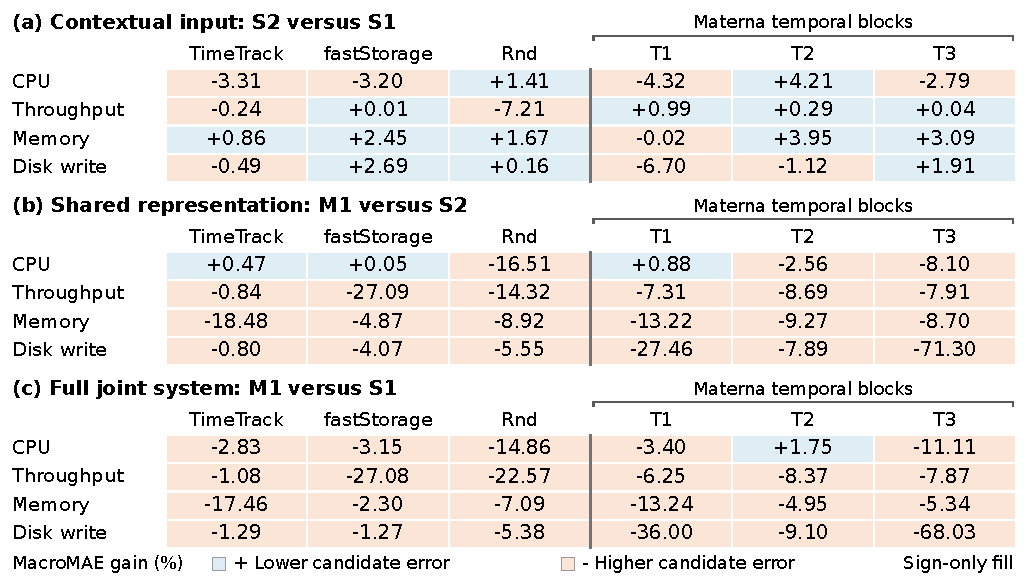
\includegraphics[width=\textwidth]{figures/results_signed_matrix.pdf}
\caption{Primary overall MacroMAE percentage gains for (a) S2 versus S1,
(b) M1 versus S2 and (c) M1 versus S1 across the evaluated evidence
blocks. Positive values indicate lower MacroMAE for the candidate
formulation; negative values indicate higher MacroMAE. Continuous signed
colour uses a symmetric $\operatorname{asinh}(G)$ mapping, with $G$ in
percentage points, as a nonlinear visual aid only. No values are clipped;
the printed raw percentages at the reported precision are authoritative.
Legend ticks are raw percentages. Colour implies neither significance nor
a consistency class. Materna T1, T2 and T3 are dependent temporal blocks.
Comparisons are bounded to the evaluated implementation and eligible
populations.}
\label{fig:primary-gains}
\end{figure*}

\subsection{RQ1 Cross-Resource Context}
\label{sec:results-rq1}

RQ1 compares independent all-resource S2 models with own-resource S1
models. Figure~\ref{fig:primary-gains}(a) shows selective
contextual value, not uniform improvement. In TimeTrack, memory was the sole
positive resource-level effect, while all four frozen classifications remained
neutral or mixed because the required consistency thresholds were not met.

The Bitbrains environments did not reproduce one common direction. In
fastStorage, memory was broadly positive and disk write conditionally positive;
CPU and throughput were neutral or mixed. The memory bootstrap interval
excluded zero, whereas the near-zero throughput interval crossed it. In Rnd,
CPU and memory were conditionally positive, while throughput and disk write
were neutral or mixed. All four Rnd intervals crossed zero, including the
interval for its negative throughput point estimate.

The Materna blocks further changed the resource pattern. T1 memory was
approximately neutral and slightly negative ($-0.02\%$); only throughput
reached the conditionally positive class. The T1 CPU interval was entirely
negative, while the other three intervals crossed zero. T2 CPU and memory
were broadly positive with intervals above zero; throughput and disk write
remained neutral or mixed. T3 memory and disk write were conditionally
positive, but all four T3 intervals crossed zero.

Memory has the clearest recurring positive pattern; the strongest benefit is
not always attached to one resource. Rnd throughput and T1 disk write illustrate
adverse effects where other blocks are near zero or positive.

\paragraph{Post-hoc cross-model and seed checks.}
The matched-context Ridge ARX:AR comparison
(Table~\ref{tab:posthoc-controls}B) also shows selective contextual value,
but individual directions depend on model family and environment. Memory
improves under Ridge in all five external blocks; fastStorage, Rnd and
Materna T2/T3 have positive point gains in both model families. TimeTrack
memory instead reverses under Ridge, and Materna T1's near-zero negative
LSTM estimate contrasts with a positive Ridge gain. Memory S2:S1 gains in
fastStorage, Rnd and Materna T2 and T3 are positive in all three recorded
seeds (Supplementary Table~S2). External memory is thus
the strongest recurring favourable contextual pattern, not a universal
benefit. Existing-seed diagnostics find sign changes in 9/24 LSTM S2:S1
block/resource summaries across the three fixed seeds (Supplementary
Table~S2). Point gains or reversals with seed-varying signs should not be
treated as seed-invariant improvements or temporal regime changes.

The Ridge TimeTrack throughput gain of $-838.45\%$ is diagnosed as
\textsc{Concentrated Degradation}, not broad Ridge failure. The saved-artifact
audit attributes $99.93\%$ of positive excess error to machine06/fold3.
ARX nevertheless improves 21/35 machine/fold pairs, with median ARX/AR MAE
ratio approximately $0.9963$. Predictions and primary MAEs are finite, and
transforms, scalers and support match the frozen design; no implementation
defect is demonstrated. The aggregate penalty must be read with this
concentration diagnosis rather than as a typical-machine effect.

\subsection{RQ2 Operational Shared-Representation Comparison}
\label{sec:results-rq2}

RQ2 compares M1 with S2, holding the all-resource input scope fixed and changing
whether the predictive representation is shared. Throughput, memory and disk
write had negative primary gains in all six blocks
(Figure~\ref{fig:primary-gains}(b)). CPU was positive only in TimeTrack,
fastStorage and Materna T1. These small or near-zero exceptions do not support
uniformly beneficial sharing within the evaluated M1 design.

In TimeTrack, memory was broadly negative; the remaining frozen resource
classifications were neutral or mixed. In fastStorage, CPU was neutral or
mixed and its bootstrap interval crossed zero. Throughput, memory and disk
write were broadly negative with intervals below zero. Rnd was broadly
negative for every resource, and each interval also lay below zero.

Materna T1 CPU was neutral or mixed with an interval crossing zero, whereas
the other resources were broadly negative with intervals wholly below zero.
T2 was broadly negative for all four resources, with entirely negative
overall intervals. In T3, throughput, memory and disk write were broadly
negative; CPU was neutral or mixed under the frozen consistency rule despite
its negative primary gain. All four T3 intervals excluded zero, with the
disk-write interval spanning $[-239.63\%,-5.94\%]$.

Degradation recurred outside the CPU exceptions, with resource- and
block-dependent magnitudes. Point signs, consistency classes and intervals
remain distinct under the frozen protocol.

\paragraph{Post-hoc sharing controls and matched cells.}
Table~\ref{tab:posthoc-controls}A shows H64 M1 against S2 constrained to the
frozen H64-M1 contexts, and H129 M1 against original S2. Throughput, memory
and disk-write point estimates remain adverse in all six blocks under both
separate controls. Context-selection freedom and the original aggregate
capacity difference are therefore incomplete explanations within this
pipeline. The controls do not identify sharing alone as the cause:
architecture, optimisation and training objectives remain part of the
implemented comparison, and common-S2 contexts align H64, not necessarily
H129. Existing-seed diagnostics find sign changes in 4/24 original M1:S2
block/resource summaries (Supplementary Table~S2), concentrated in small
CPU exceptions and TimeTrack throughput. Adverse aggregate directions do not
imply adverse outcomes for every seed. Here, ``stable'' means ``no sign flip
across the three recorded seeds''. Sign stability does not imply magnitude
stability: Materna T3 M1:S2 disk-write gains are $-54.65\%$, $-71.55\%$ and
$-87.84\%$ (Supplementary Table~S2).

The post-hoc matched-cell diagnostics further separate direction from
magnitude. A cell is entity $\times$ outer fold $\times$ forecast lead, with
MAE first averaged across existing seeds. In all 24 original M1:S2
block/resource summaries (Supplementary Table~S1), the median candidate/reference MAE ratio exceeds
one and the candidate win rate is below $50\%$. This includes the small
positive CPU MacroMAE exceptions. Materna T1/T3 disk-write median ratios are
approximately $1.0246/1.0347$, despite MacroMAE gains of
$-27.46\%/-71.30\%$. The adverse typical-cell direction is widespread, but
the much larger mean-error penalties do not describe every VM or the
magnitude of degradation in a typical cell.

Post-hoc attribution locates this uneven magnitude. In Materna T1/T3,
28/35 and 32/35 VM-averaged disk-write errors worsen. VM266 dominates the T1
tail and VM272 the T3 tail, contributing 82.10\% and 86.97\% of positive
excess error, respectively; the top three VMs contribute 91.72\% and 92.93\%.
No training or scaling defect was demonstrated. A post-hoc frozen-partition
audit, using each VM's frozen M1-selected context within each fold, places
their log-space training IQRs near the upper cohort tail: VM266 ranks
33--34/35 at approximately 7.86--8.19 times the cohort median IQR, and VM272
ranks 35/35 at 7.59--7.75 times it. Both have the largest native disk-write
IQR in every fold. Unusually small training IQRs are therefore not supported as an
explanation for these tails. This does not establish that the large scale
caused the errors or that sharing is causal.
For TimeTrack memory, all seven machine averages and 31/35 machine/fold
pairs worsen, with median pair ratio $1.195276$. The largest pair contributes
21.80\% and the top three 51.06\% of positive excess error at that same
machine/fold level. Adverse direction is broad but magnitude uneven;
pair-level attribution must not be
conflated with the finer matched-cell medians in Supplementary Table~S1.

% Formatting-only projection of authoritative post-hoc CSV fields.
\begin{table*}[t]
  \caption{POST-HOC sensitivity comparisons alongside frozen reference gains (\%).}
  \label{tab:posthoc-controls}
  \centering
  \small
  \setlength{\tabcolsep}{2pt}
  \renewcommand{\arraystretch}{1.12}
  \begin{tabular*}{\textwidth}{@{\extracolsep{\fill}}lrrrr@{}}
    \toprule
    \multicolumn{5}{l}{\textbf{A:} [H64 M1:S2 / H64 M1:common-S2 / H129 M1:S2]} \\
    Block & CPU & Throughput & Memory & Disk write \\
    \midrule
    TimeTrack & $[+0.47/-0.81/-2.93]$ & $[-0.84/-0.54/-0.16]$ & $[-18.48/-17.79/-18.48]$ & $[-0.80/-0.56/-0.60]$ \\
    fastStorage & $[+0.05/+0.36/+3.14]$ & $[-27.09/-20.31/-33.83]$ & $[-4.87/-4.43/-4.19]$ & $[-4.07/-1.75/-4.05]$ \\
    Rnd & $[-16.51/-16.32/-17.57]$ & $[-14.32/-12.57/-15.56]$ & $[-8.92/-8.69/-8.06]$ & $[-5.55/-3.72/-6.85]$ \\
    Materna T1 & $[+0.88/-0.61/+3.19]$ & $[-7.31/-7.19/-4.72]$ & $[-13.22/-10.15/-12.32]$ & $[-27.46/-27.98/-24.62]$ \\
    Materna T2 & $[-2.56/-1.38/+0.17]$ & $[-8.69/-7.26/-3.65]$ & $[-9.27/-7.52/-6.72]$ & $[-7.89/-7.93/-7.20]$ \\
    Materna T3 & $[-8.10/-7.40/-8.21]$ & $[-7.91/-7.44/-5.83]$ & $[-8.70/-7.79/-6.53]$ & $[-71.30/-69.67/-64.00]$ \\
    \midrule
    \multicolumn{5}{l}{\textbf{B:} [frozen LSTM S2:S1 / Ridge ARX:AR]} \\
    Block & CPU & Throughput & Memory & Disk write \\
    \midrule
    TimeTrack & $[-3.31/-14.00]$ & $[-0.24/-838.45]$\textsuperscript{a} & $[+0.86/-23.21]$ & $[-0.49/-7.58]$ \\
    fastStorage & $[-3.20/-4.37]$ & $[+0.01/-20.75]$ & $[+2.45/+2.88]$ & $[+2.69/+1.05]$ \\
    Rnd & $[+1.41/+0.22]$ & $[-7.21/+0.37]$ & $[+1.67/+4.26]$ & $[+0.16/+1.68]$ \\
    Materna T1 & $[-4.32/+6.27]$ & $[+0.99/-13.90]$ & $[-0.02/+7.22]$ & $[-6.70/+2.05]$ \\
    Materna T2 & $[+4.21/+9.67]$ & $[+0.29/+0.91]$ & $[+3.95/+6.47]$ & $[-1.12/+10.07]$ \\
    Materna T3 & $[-2.79/+2.17]$ & $[+0.04/-2.15]$ & $[+3.09/+1.81]$ & $[+1.91/-0.69]$ \\
    \bottomrule
  \end{tabular*}
  \vspace{2pt}
  \parbox{\textwidth}{\footnotesize Positive means lower candidate MacroMAE; values are rounded to two decimals.
  Frozen H64 M1:S2 and LSTM S2:S1 references are repeated unchanged, not replaced by controls.
  For TimeTrack memory, both H64 and H129 gains round to $-18.48\%$; they are distinct before rounding.
  Common-S2 uses H64-M1 contexts; H129 selects its own contexts. These are separate controls, not joint causal isolation.
  \textsuperscript{a}The TimeTrack Ridge throughput penalty is concentrated in machine06/fold3:
  99.93\% of positive excess error; ARX improves 21/35 machine/fold pairs, median ARX/AR ratio $0.9963$ (Section~\ref{sec:results-rq1}).
  Point signs imply neither significance nor model-independent benefit; Materna T1--T3 remain dependent blocks.}
\end{table*}


\subsection{RQ3 Full Joint-System Performance}
\label{sec:results-rq3}

RQ3 compares the complete M1 system with local-resource S1 models.
Figure~\ref{fig:primary-gains}(c) is negative in every displayed cell except
Materna T2 CPU, so the full joint formulation generally did not outperform S1.
In TimeTrack, memory and disk write were broadly negative; CPU and throughput
were neutral or mixed under the prospective consistency criteria.

In fastStorage, CPU and throughput were broadly negative, whereas memory and
disk write were neutral or mixed. The throughput interval was entirely below
zero, while the other three overall intervals crossed zero. In Rnd, every
resource was broadly negative and every interval lay below zero.

In Materna T1, throughput and disk write were broadly negative; CPU and memory
were neutral or mixed, although all four VM-cluster intervals lay below zero.
The T2 CPU exception ($+1.75\%$) was conditionally positive, but its interval
crossed zero ($[-3.52\%,+6.07\%]$). T2 disk write was broadly negative, and
throughput and memory were neutral or mixed. In T3, CPU, throughput and disk
write were broadly negative, while memory was neutral or mixed; only the
memory interval narrowly crossed zero. These differences in classification
and uncertainty remain important despite the nearly uniform negative sign
pattern.

RQ3 combines both design changes. Its gains are reported directly, not added
from RQ1 and RQ2 percentages (Section~\ref{sec:decomposition}).

\subsection{RQ4 Resource, Environment, and Temporal Heterogeneity}
\label{sec:results-rq4}

Figure~\ref{fig:primary-gains} reveals heterogeneity at each prespecified
level. Resource heterogeneity is evident in the selective S2-versus-S1
benefits and changing resource ordering. CPU, throughput and disk write change
direction across evidence blocks, whereas memory is positive in five and
nearly zero and negative only in Materna T1. Repeated positive memory effects
therefore do not imply invariant resource behaviour.

External-environment heterogeneity is stronger for representation sharing: fastStorage
CPU was near zero while the other three resources were negative; Rnd was
broadly negative for all four. Temporal heterogeneity within the dependent
Materna blocks is distinct: M1-versus-S2 CPU changed from positive in T1 to
negative in T2--T3, moving from neutral or mixed to broadly negative and back
to neutral or mixed. Throughput, memory and disk write were broadly negative
in all three Materna blocks, with varying magnitudes. For M1 versus S1, CPU
alone reversed sign in T2; throughput and disk write stayed negative and
memory stayed negative but neutral or mixed across T1--T3.

Sign, magnitude, and frozen class capture different aspects of this
heterogeneity. For example, T3 S2-versus-S1 throughput was slightly positive at
$+0.04\%$ but remained neutral or mixed, while T2 CPU was both positive and
broadly positive. T3 M1-versus-S2 CPU had a negative point estimate and an
interval below zero, yet remained neutral or mixed under the separate
consistency rule. These combinations prevent near-zero sign changes from being
treated as equivalent to changes supported across the prescribed units. They
also show why the within-Materna decision uses the frozen classification and
trace rules alongside the raw gains.

The frozen within-Materna RQ4 outcome was recorded as follows.

\noindent The prespecified RQ4 criterion for temporal heterogeneity was met.
Seven of the 12
resource--comparison pairs changed frozen classification across T1--T3 and
five changed raw sign. The S2-versus-S1 trace decision also changed: T1 met the
frozen non-support rule, whereas T2 and T3 were mixed. The M1-versus-S2
trace-level decision was consistently not supported, even though its CPU
classification varied. Several small S2 effects are seed-variable
(Supplementary Table~S2). This is a descriptive criterion, not an IID or
inferential claim; no post-hoc temporal regimes or causal mechanisms are
inferred.

\subsection{Persistence Boundary}
\label{sec:results-persistence}

Relative formulation gains do not establish superiority to a persistence
forecast. In TimeTrack, S1, S2, and M1 all had positive mean persistence skill
for throughput and disk write, and their CPU means were also positive. Memory
was the boundary: mean skill was $-0.1272$ for S1, $-0.1494$ for S2, and
$-0.6047$ for M1, with positive skill at only two, four, and zero of eight
leads. Thus the large negative M1-versus-S2 memory result coincided with weak
absolute performance relative to persistence, whereas the throughput and
disk-write formulation comparisons occurred in resources with positive
average absolute skill.

Neither Bitbrains environment contained a formulation that beat persistence
for every resource. Overall CPU skill was negative for S1, S2, and M1 in both
environments. In fastStorage, throughput skill was also negative for every
formulation; memory and disk write were positive for all three. Rnd again had
positive memory and disk-write skill for all formulations, while throughput
was only slightly positive for S1 ($0.0384$) and negative for S2 ($-0.0257$)
and M1 ($-0.1176$). Consequently, a positive S2-versus-S1 gain for Rnd CPU or a
relative degradation under M1 does not by itself describe absolute forecasting
skill.

Materna showed a different aggregate boundary. S2 beat persistence in all 12
trace--resource overall aggregates. No formulation, however, beat persistence
in every individual trace--resource--lead cell. At the overall level, M1 failed
the check for T1 throughput ($-0.0608$), T1 disk write ($-1.7590$), T3
throughput ($-0.2629$), and T3 disk write ($-1.3493$); it remained positive for
all four T2 resources. S1 additionally failed only T1 throughput at the overall
level, while S2 had no overall failures. These persistence results delimit
absolute forecasting performance and remain separate from the controlled
S1--S2--M1 comparisons.

Thus relative gain, overall persistence skill and horizon-level skill answer
different questions (Section~\ref{sec:evaluation}); none establishes uniform
absolute forecasting superiority.

\subsection{Accuracy-Efficiency Trade-Off}
\label{sec:results-efficiency}

The original H64 M1 consolidates the target-model complement for one entity,
outer fold and seed (Table~\ref{tab:efficiency}). In the five-horizon external design, S1 uses four
networks and 203,028 parameters, S2 four networks and 206,100 parameters, and
M1 one joint network and 52,500 parameters: approximately $74.5\%$ fewer
parameters and $75\%$ fewer models than S2. TimeTrack's eight-horizon
complements contain 206,880 S2 parameters and 53,280 M1 parameters. These
are local architecture inventories, not a globally deployed four-versus-one
system or total training-fit counts. The post-hoc H129 comparison changes
the parameter budget and must not inherit H64's parameter-reduction claim.

% Five-horizon parameter counts and frozen Materna execution accounting.
\begin{table}[t]
  \caption{Model consolidation and observed Materna fitting cost.}
  \label{tab:efficiency}
  \centering
  \small
  \begin{tabular}{@{}lrrr@{}}
    \toprule
    Formulation & Models & Parameters & Fit-hours \\
    \midrule
    S1 & 4 & 203,028 & 85.59 \\
    S2 & 4 & 206,100 & 75.30 \\
    M1 & 1 &  52,500 & 20.41 \\
    \bottomrule
  \end{tabular}

  \vspace{2pt}
  \parbox{\columnwidth}{\footnotesize Parameter counts refer to the
  five-horizon external instantiation. Fit-hours are observed totals from the
  three Materna traces. Relative to S2, M1 uses approximately 74.5\% fewer
  parameters and 75\% fewer models.}
\end{table}


The frozen Materna totals are 85.594240 worker fit-hours for S1, 75.303186 for
S2 and 20.405083 for M1. As defined in Section~\ref{sec:architecture-training},
these sum successful inner-candidate and final-refit durations, including
inner validation, across the three traces. They are not elapsed wall time,
energy, deployment cost or production latency. Different executed epochs and
selected contexts can contribute to the S1--S2 order; input width alone does
not explain it. The measured training workload and local model consolidation
coexist with the accuracy penalties above, without establishing production
savings or an architecture-independent efficiency ranking.

\section{Cross-Dataset Synthesis}
\label{sec:cross-dataset-synthesis}

Table~\ref{tab:cross-study-synthesis} retains frozen TimeTrack,
equal-environment Bitbrains and equal-temporal-block Materna summaries under
Section~\ref{sec:replication-design}, without a global score.
The post-hoc evidence in Sections~\ref{sec:results-rq1}--\ref{sec:results-rq2}
qualifies their interpretation; agreement concerns operational directions,
not independent replication of a sharing mechanism.

% Frozen cross-study descriptive synthesis from the Phase 4D final freeze.
% Bitbrains and Materna columns are equal-block summaries; no source pooling.
\begin{table*}[t]
  \caption{Frozen descriptive source summaries of primary overall MacroMAE
  gain (\%).}
  \label{tab:cross-study-synthesis}
  \centering
  \small
  \setlength{\tabcolsep}{3pt}
  \begin{tabular*}{\textwidth}{@{\extracolsep{\fill}}l*{9}{r}@{}}
    \toprule
    & \multicolumn{3}{c}{S2 versus S1}
      & \multicolumn{3}{c}{M1 versus S2}
      & \multicolumn{3}{c}{M1 versus S1} \\
    \cmidrule(lr){2-4}\cmidrule(lr){5-7}\cmidrule(l){8-10}
    Resource & TimeTrack & Bitbrains & Materna
      & TimeTrack & Bitbrains & Materna
      & TimeTrack & Bitbrains & Materna \\
    \midrule
    CPU & $-3.31$ & $-0.89$ & $-0.97$
      & $0.47$ & $-8.23$ & $-3.26$
      & $-2.83$ & $-9.01$ & $-4.25$ \\
    Throughput & $-0.24$ & $-3.60$ & $0.44$
      & $-0.84$ & $-20.71$ & $-7.97$
      & $-1.08$ & $-24.82$ & $-7.50$ \\
    Memory & $0.86$ & $2.06$ & $2.34$
      & $-18.48$ & $-6.89$ & $-10.40$
      & $-17.46$ & $-4.70$ & $-7.85$ \\
    Disk write & $-0.49$ & $1.42$ & $-1.97$
      & $-0.80$ & $-4.81$ & $-35.55$
      & $-1.29$ & $-3.33$ & $-37.71$ \\
    \bottomrule
  \end{tabular*}

  \vspace{2pt}
  \parbox{\textwidth}{\footnotesize
    Positive values indicate lower MacroMAE for the candidate formulation;
    negative values indicate higher MacroMAE. TimeTrack: development summary.
    Bitbrains: equal-environment synthesis of fastStorage and Rnd.
    Materna: equal-temporal-block synthesis of T1--T3, consecutive dependent
    temporal blocks rather than independent replications. Comparisons are
    descriptive, without cross-source aggregation.}
\end{table*}


\subsection{TimeTrack}

TimeTrack's small positive S2:S1 memory and M1:S2 CPU estimates vary across
seeds. Ridge reverses the contextual memory direction; its throughput penalty
is concentrated in one machine/fold (Section~\ref{sec:results-rq1}).
This is development evidence, not independent external confirmation.

\subsection{Bitbrains External Confirmation}

Memory has favourable LSTM/Ridge contextual point agreement in both external
environments, whereas throughput reverses direction between families in each.
Their equal-environment summary must not erase these block-specific differences.

\subsection{Materna Temporal Replication}

LSTM/Ridge memory gains agree favourably in T2/T3, but T1's near-zero,
seed-variable LSTM estimate contrasts with positive Ridge gain. Other resource
directions depend on block and family. These consecutive blocks retain the
same selected VM identifiers; their dependence and the T1/T3 disk-write
magnitude qualifications (Section~\ref{sec:results-rq2}) preclude independent
replication or uniformly severe VM-degradation claims.

\subsection{Generalisation Boundaries}

\paragraph{Contextual inputs.}
External memory recurs favourably, but cross-family reversals and seed-variable
small effects require resource-, environment- and family-specific validation.

\paragraph{Shared representation.}
Both separate controls retain adverse throughput, memory and disk-write
points. Median MAE ratios and win rates retain the adverse typical-cell
direction despite small positive CPU MacroMAE gains. Capacity and selection
are incomplete explanations, not eliminated causal factors
(Section~\ref{sec:results-rq2}).

\paragraph{Complete joint system and consolidation.}
M1:S1 gains are negative except Materna T2 CPU. Local model counts and worker
fit-hours describe a consolidation/workload trade-off, not production benefit
(Section~\ref{sec:results-efficiency}). Population, model-family, seed and
persistence limits are assessed in Section~\ref{sec:threats}; the controls
neither change the endpoints nor extend evidence to excluded VMs or untested
shared architectures.

\section{Discussion}
\label{sec:discussion}

\subsection{When Cross-Resource Context Helps}
\label{sec:discussion-context}

Cross-family agreement for external memory, TimeTrack's reversal and T1's
seed-variable estimate support selective contextual value, not a universal
memory benefit (Section~\ref{sec:results-rq1}). Small seed-variable effects
cannot establish stable improvements or temporal regimes.

This agrees with MMRP's non-uniform contextual gains \citep{Tripathi2025MMRP}
and the relevance of environment-specific evaluation
\citep{Rossi2025CloudUncertainty}. TimeTrack correlations
\citep{Meliani2025TimeTrack} motivate inputs, not conditional predictive value
or causal resource coupling.

The concentrated Ridge throughput penalty in Section~\ref{sec:results-rq1}
shows why a large aggregate loss must not be generalised to typical-machine
failure; the saved-artifact checks demonstrated no implementation defect.

\subsection{Shared Representation and Adverse Transfer}
\label{sec:discussion-sharing}

The separate sensitivity controls retain adverse throughput, memory and
disk-write points across all six blocks (Section~\ref{sec:results-rq2}).
Context selection and aggregate capacity contribute to magnitudes but do not
suffice to explain the pattern.

Direction need not imply uniform severity. Materna T1/T3 disk-write median
ratios are about $1.025/1.035$, despite much larger tail-sensitive MacroMAE penalties.
Direction is broadly adverse but absolute-error magnitude concentrated,
not equally severe in every VM (Section~\ref{sec:results-rq2}).

The outcome is operationally consistent with adverse transfer, not a uniquely
identified sharing mechanism. Useful task-dependent transfer is established
\citep{Caruana1997Multitask,Standley2020TaskGrouping,Fifty2021TaskGroupings},
including in forecasting \citep{Nikentari2022NARMAXLSTM,Nochumsohn2025MTLinear}.
Gradient conflict, representation interference and capacity competition were
not measured. Nominal loss weights do not establish realised contributions
(Section~\ref{sec:m1}); architecture, optimisation and selection remain coupled.
Multi-objective or gradient-aware designs
\citep{Sener2018MultiObjective,Yu2020GradientSurgery} are alternatives, not
diagnoses or demonstrated remedies for these models.

\subsection{Implications for Runtime and Cloud Software Systems}
\label{sec:discussion-systems}

Forecasting supports adaptation \citep{Taherizadeh2018Monitoring,Bauer2020SelfAware},
but adding telemetry and consolidating predictors require separate resource-
and horizon-specific validation on future-only support, including persistence
(Section~\ref{sec:results-persistence}). A contextual benefit does not imply a
sharing benefit. Controller outcomes depend on policy and platform
\citep{Qu2018Autoscaling}; no autoscaler, scheduler or controller was deployed.
Production latency, energy, monetary savings, SLA improvements and controller
benefits were not measured.

\subsection{Accuracy-Consolidation Trade-Off}
\label{sec:discussion-efficiency}

The local H64 model/parameter reductions and lower Materna worker fit-hours
coexist with accuracy losses (Section~\ref{sec:results-efficiency}).
H129 retains consolidation but not H64's parameter reduction. Compactness is
therefore a trade-off, not a free predictive gain. Joint accuracy/computation
assessment follows task-grouping and service-forecasting research
\citep{Standley2020TaskGrouping,Syu2017DynamicQoS}; deployment still requires
platform measurements and resource-specific error tolerances.

Per-entity consolidation may still be attractive where modest target-specific
accuracy penalties are acceptable. This requires distinguishing typical-cell
magnitude from tail-sensitive MacroMAE penalties and checking adverse tails,
not recommending M1 universally or treating concentrated excess as irrelevant.

\subsection{Applicability and Generalisation Limits}
\label{sec:discussion-applicability}

The population and dependence limits in Sections~\ref{sec:population-restrictions}
and~\ref{sec:threats-external} bound applicability. Cross-family reversals do not
select a universal replacement. Selective grouping and adaptive or hybrid
sharing remain untested alternatives
\citep{Fifty2021TaskGroupings,Yu2020GradientSurgery,Nochumsohn2025MTLinear}.
Global models remain outside this evaluation
\citep{MonteroManso2021GlobalForecasting}.
The same limit applies to foundation forecasters
\citep{DiMenna2026RuntimeForecasting}. Future comparisons should retain
independent all-input controls and resource-specific assessment while
measuring proposed mechanisms.

\section{Threats to Validity}
\label{sec:threats}

\subsection{Construct Validity}
\label{sec:threats-construct}

The three formulations are not a complete $2\times2$ design. Original
capacity/context differences are addressed separately, not jointly, by the
post-hoc controls (Section~\ref{sec:posthoc-controls}). H129's fresh selection
and H64-aligned common-S2 contexts leave residual differences; parameter-count
proximity is not architectural, task-capacity or optimisation equivalence.

CPU, throughput, memory and disk-write mappings have source-specific
definitions and native units, not perfect measurement equivalence.
MacroMAE gains describe the specified error estimand; RMSE, $R^2$, native
NMAE and persistence provide complementary diagnostics. Metric choice can
alter rankings \citep{Hyndman2006Accuracy}. Scaled-space training and selection
objectives are distinct from native-unit evaluation
(Sections~\ref{sec:model-selection}--\ref{sec:evaluation}), and a relative
formulation gain need not establish useful absolute skill.

\subsection{Internal Validity}
\label{sec:threats-internal}

The chronology, purging and training-only preprocessing in
Section~\ref{sec:leakage-control} constrain leakage
\citep{Cerqueira2020Evaluation,Hyndman2021Forecasting}.
Matched support and provenance cannot exclude all implementation/data errors.
Original external criteria were prospective; reviewer-motivated controls are
post-hoc, not prespecified confirmation.

Only three neural seeds were recorded. Existing diagnostics identify 9/24
S2:S1 and 4/24 M1:S2 block/resource summaries whose gains change sign across
those seeds (Supplementary Table~S2). These counts do not establish a general noise floor or stability
under arbitrary retraining. Contexts, epochs and optimisation can interact
with formulation, and missing gradient/clipping histories limit mechanism
attribution even after the separate controls.

Ridge is deterministic but restricted to a finite five-alpha grid and frozen
H64-M1 contexts, which were selected for the LSTM design rather than optimised
for Ridge. Boundary alpha selections do not establish performance under a
wider regularisation search. Its selection uses native-unit validation MAE,
unlike the LSTM context score, so cross-family disagreement is conditional on
these implemented designs, not an architecture-only intervention.

\subsection{External Validity}
\label{sec:threats-external}

The sources represent particular runtime/cloud contexts, not probability
samples of all VMs. Excluded workloads may differ
(Section~\ref{sec:population-restrictions}). Materna's shared source and VM
identifiers make temporal agreement repeated-within-source evidence, not
independent-dataset replication.

The evaluated model families comprise the conventional LSTM formulations,
their width/context controls and the matched-context Ridge pair. Reversals
across these designs preclude model-independent contextual claims.
Transformers, mixture-of-experts, selective grouping, adaptive sharing,
gradient surgery and foundation forecasters were not tested. Four resource
semantics do not establish accuracy for application latency, queue lengths,
QoS or downstream SLA outcomes.

\subsection{Conclusion Validity}
\label{sec:threats-conclusion}

MacroMAE weights seed-averaged entity--fold cells and horizons equally, but
large native errors affect it differently from median ratios and win rates.
The direction/magnitude distinction in Section~\ref{sec:results-rq2} precludes
uniform VM-level interpretations; diagnostics do not replace primary estimates.

Paired VM-cluster bootstrap intervals condition on the evaluated external
cohorts and protocol. They are separate from frozen consistency classes and
point signs, not classical significance claims or intervals retrospectively
assigned to every post-hoc control. Overlapping expanding folds, multiple
horizons, repeated seeds and dependent Materna blocks are not IID replicates.
No six-block global effect, independent-dataset meta-analysis or IID
interpretation is used to strengthen these conclusions.

Persistence failures in Section~\ref{sec:results-persistence} limit absolute
skill claims. Neither relative gains nor descriptive source summaries support
a universal verdict beyond the evaluated formulations and populations.

\section{Conclusion}
\label{sec:conclusion}

Contextual input and representation sharing require separate design decisions.
External memory recurs favourably, but Ridge and seed sensitivity bound
contextual value by model and environment. The evaluated shared-LSTM model
generally loses throughput, memory and disk-write accuracy while consolidating
per-entity models. Adverse point directions survive separate post-hoc common-context
and H129 approximate-capacity controls, without identifying sharing alone as
the mechanism. Typical-cell penalties can be more modest than tail-sensitive
MacroMAE suggests: per-entity consolidation may be attractive when
target-specific accuracy penalties are acceptable, provided adverse tails
are assessed. These findings do not universally reject multi-task forecasting.
Validate contextual input and consolidation by resource and design, within
the eligible population and against absolute persistence skill.

\section*{Data availability}

TimeTrack is publicly available on
\href{https://www.kaggle.com/datasets/abdelghanimeliani/open-air-interface-cicd-timeseries-dataset}{Kaggle}
(Apache 2.0 in its dataset metadata) and in the publisher's
\href{https://doi.org/10.5281/zenodo.15442251}{Zenodo archive
(doi:10.5281/zenodo.15442251; CC BY 4.0)}; its description paper is
\citet{Meliani2025TimeTrack}. These are source-specific licence statements.
Bitbrains fastStorage and Rnd are publicly available as
\href{https://atlarge-research.com/gwa-t-12/}{GWA-T-12}
\citep{Shen2015Bitbrains}; Materna T1--T3 are publicly available as
\href{https://atlarge-research.com/gwa-t-13/}{GWA-T-13}
\citep{Kohne2014FederatedCloudSim,Kohne2016SLAScheduling}.
We acknowledge Bitbrains IT Services Inc. and Materna GmbH Information
\& Communications, respectively, for providing these traces through the
Grid Workloads Archive. Their separate source pages specify acknowledgement
and citation conditions, rather than a standard open-data licence. Readers
should obtain third-party raw data from these original sources and consult
each source's terms before redistribution.

Source code, protocols, derived analysis outputs and SHA-256 inventories are
publicly accessible in the
\href{https://github.com/KADOUMAAbdelhak/TimeTrack-Forecasting-Framework/tree/fee20c316040c57b69ba12a193530c955b539771}{project repository at scientific checkpoint \texttt{fee20c3}}.
The public checkpoint does not include the full fitted-model or per-fit
prediction collections; the checksum inventories do not themselves provide
those files. No repository-wide reuse licence is asserted here.

\printcredits

\section*{Funding}

This research did not receive any specific grant from funding agencies in
the public, commercial, or not-for-profit sectors.


\bibliographystyle{cas-model2-names}
\bibliography{references}

\end{document}
